\section{Pollution}

\begin{multicols}{2}


\subsection{Pollution and Chemistry}

\begin{center}
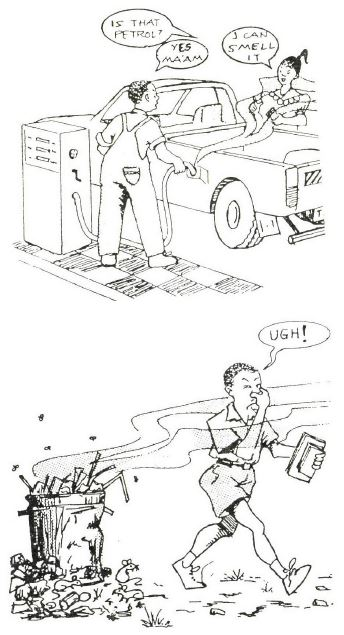
\includegraphics[width=0.4\textwidth]{./img/source/air-pollution.jpg}
\end{center}

\begin{description*}
%\item[Subtopic:]{}
%\item[Materials:]{}
%\item[Setup:]{}
\item[Procedure:]{Divide the class into small groups. Think of some daily situations where pollution is seen in air, water or soil. Write them out on cards and give one to each group of students. One by one, have a group read the situation and then ask the class what kind of pollution is present and what suggestions they can give on how to reduce pollution in that situation.}
%\item[Hazards:]{}
%\item[Questions:]{}
%\item[Observations:]{}
%\item[Theory:]{}
%\item[Applications:]{}
%\item[Notes:]{}
\end{description*}

\section*{Terrestrial Pollution}


\subsection{Trash Journal} % Shika 242 

%\begin{center}
%\includegraphics[width=0.4\textwidth]{./img/.png}
%\end{center}

\begin{description*}
%\item[Subtopic:]{}
%\item[Materials:]{}
%\item[Setup:]{}
\item[Procedure:]{Have each student record in a journal all of the trash that they make every day for 2 weeks. If possible, collect the trash and weigh it every day.}
%\item[Hazards:]{}
\item[Observations:]{}
\item[Theory:]{Trash is a big problem in large towns and cities. Many manufactured goods come with a lot of waste material, which accumulates over time. Many waste items can be \emph{recycled}, or reused for different purposes.}
\item[Questions:]{What are some methods for eliminating waste? What effect does burning trash have on the environment?}
%\item[Applications:]{}
%\item[Notes:]{}
\end{description*}

\subsection{Biodegradable Waste} % banana, bottle, etc in a hole

%\begin{center}
%\includegraphics[width=0.4\textwidth]{./img/.png}
%\end{center}

\begin{description*}
%\item[Subtopic:]{}
\item[Materials:]{Shovel/jembe, Banana peel, plastic bottle, rubber bands, paper}
%\item[Setup:]{}
\item[Procedure:]{Dig several small holes and place a different item in each, covering them with dirt. Check back on the items after several weeks, months, and after a year.}
%\item[Hazards:]{}
%\item[Questions:]{}
\item[Observations:]{The banana peel shrivels and degrades after a couple weeks, while the other items remain for many months or even years.}
\item[Theory:]{Banana peels are an example of organic waste. They are \emph{biodegradable}}, meaning that it breaks down in the environment. \emph{Non-biodegradable} waste does not break down, it just piles up.
\item[Applications:]{Do not throw plastic bottles out of the window on buses!!}
%\item[Notes:]{}
\end{description*}

\subsection{Planting Trees}

\begin{center}
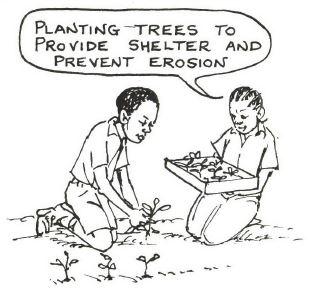
\includegraphics[width=0.4\textwidth]{./img/source/planting-trees.jpg}
\end{center}

\begin{description*}
%\item[Subtopic:]{}
%\item[Materials:]{}
%\item[Setup:]{}
\item[Procedure:]{Planting trees and protecting newly planted trees from animals is one way for community members to look out for the well-being of their environment and maintain and beautify their homes and schools.}
%\item[Hazards:]{}
%\item[Questions:]{}
%\item[Observations:]{}
\item[Theory:]{Trees consume excess carbon dioxide, which is a harmful greenhouse gas that eats away at our ozone layer. They produce the oxygen that we breath and help to maintain a balanced ecosystem for other organisms. }
\item[Applications:]{Many individuals cut down trees for firewood but fail to replace them with newly planted trees. Over time this can lead to erosion and degradation of the land.}
%\item[Notes:]{}
\end{description*}

\columnbreak

%\vfill

%==================================================================================================%

\section*{Water Pollution}


\subsection{Water Purity Surveys}

\begin{center}
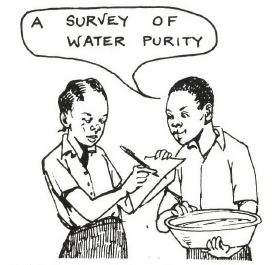
\includegraphics[width=0.4\textwidth]{./img/source/water-purity.jpg}
\end{center}

\begin{description*}
%\item[Subtopic:]{}
%\item[Materials:]{}
%\item[Setup:]{}
\item[Procedure:]{Keeping a record of water purity and health in a local community is a great way to raise awareness about environmental protection. Students can test for hardness of water, pH, or other impurities and harmful bacteria present in water samples.}
%\item[Hazards:]{}
\item[Questions:]{What are some other ways that you can get involved in protecting the environment?}
%\item[Observations:]{}
%\item[Theory:]{}
%\item[Applications:]{}
%\item[Notes:]{}
\end{description*}

\subsection{Acid Rain}

\begin{center}
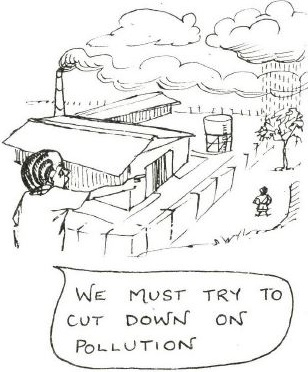
\includegraphics[width=0.35\textwidth]{./img/source/acid-rain.jpg}
\end{center}

\begin{description*}
%\item[Subtopic:]{}
%\item[Materials:]{}
%\item[Setup:]{}
%\item[Procedure:]{}
%\item[Hazards:]{}
%\item[Questions:]{}
%\item[Observations:]{}
%\item[Theory:]{}
\item[Applications:]{Pollution (e.g. from factories and cars) is carried in the wind and eventually lowers the pH of the water droplets in the air. Eventually the water returns to the ground as acid rain. The acid rain may fall a long way from the cause of the pollution - often in a different country.}
%\item[Notes:]{}
\end{description*}

\columnbreak

%==================================================================================================%

\section*{Air Pollution} % CO2, NOx, CFCs, smog, acid rain


\subsection{Smog}

\begin{center}
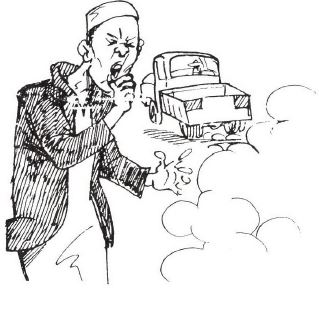
\includegraphics[width=0.35\textwidth]{./img/source/pollution-smog.jpg}
\end{center}

\begin{description*}
%\item[Subtopic:]{}
%\item[Materials:]{}
%\item[Setup:]{}
%\item[Procedure:]{}
%\item[Hazards:]{}
%\item[Questions:]{}
\item[Observations:]{On sunny days, nitrogen oxides react with other
pollutants of the air to form smog. You may be
able to observe smog on sunny days over large
cities if you look from a tall building or a
mountain.}
\item[Theory:]{Everywhere combustion at high temperature
takes place in air, nitrogen from the air reacts
with oxygen to form various nitrogen oxides.
They are present in the exhaust from cars,
lorries and buses, in the smoke of burning
charcoal etc. Smog damages the lungs of people,
especially children and old people, and the
tissues of plants.}
%\item[Applications:]{}
%\item[Notes:]{}
\end{description*}

%==================================================================================================%

\section*{Global Warming} % greenhouse effect


\subsection{Greenhouse Bucket}

%\begin{center}
%\includegraphics[width=0.4\textwidth]{./img/.png}
%\end{center}

\begin{description*}
%\item[Subtopic:]{}
\item[Materials:]{Buckets, black paint/shoe polish, sheet of glass, water}
%\item[Setup:]{}
\item[Procedure:]{Get two dark coloured buckets or paint them black on the outside. Fill them with water and place them out in the sun on a hot day. Place a sheet of glass over the top of one of the buckets. At the end of the day feel the water in the two buckets.}
%\item[Hazards:]{}
%\item[Questions:]{}
\item[Observations:]{The bucket with the glass sheet covering will be warmer.}
\item[Theory:]{The glass allows light rays to enter through it, but reflects some of its energy back into the bucket as it tries to escape. Hence the light and heat are trapped inside the bucket and the water temperature increases. }
\item[Applications:]{When the sun heats the surface of the earth it
sends back heat radiation into the atmosphere.
Carbon dioxide and the other greenhouse gases
form a blanket which does not allow the radiant
heat to escape. Thus the temperature of the
atmosphere is gradually increasing making the
earth warmer.}
%\item[Notes:]{}
\end{description*}

%\subsection{The Greenhouse Effect}
%
%\begin{center}
%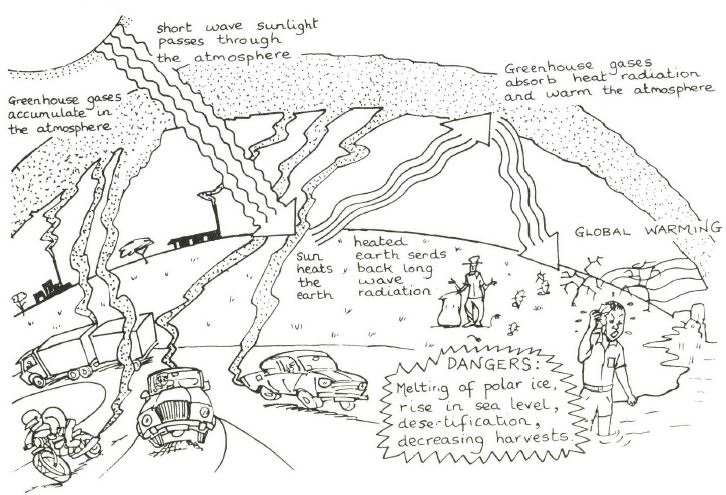
\includegraphics[width=0.95\textwidth]{./img/source/greenhouse-effect.jpg}
%\end{center}
%
%\begin{description*}
%%\item[Subtopic:]{}
%\item[Materials:]{}
%\item[Setup:]{}
%\item[Procedure:]{}
%\item[Hazards:]{}
%\item[Questions:]{}
%\item[Observations:]{}
%\item[Theory:]{}
%\item[Applications:]{}
%\item[Notes:]{}
%\end{description*}


\end{multicols}

\pagebreak